
\section{Design}
\label{sec:design}

\begin{comment}   
Pattern matching algorithms require the input stream of events to be
(partially) sorted on time, while this is not always the case in practice due
to competing constraints of other stages in the data processing pipeline. 
\end{comment}
Evaluating pattern matching queries in a map-reduce framework usually 
adds a reduction step in order to sort the input, which can become the main 
bottleneck of the workload, both at the network level (large amounts of 
shuffled data) and at the processing level.
The standard approach to minimize the cost of sorting/data shuffling has been 
to introduce a {\em preprocessing} phase which first filters the input based on 
the {\em selection} predicates, i.e.\ removes all events that do not satisfy 
the guard of at least one event variable while ignoring its {\em join} 
predicates.
This {\em preprocessing} phase can significantly reduce both processing costs 
and latency since it takes linear time in the size of the input (as opposed to 
$O(nlogn)$ for sorting) and is embarrassingly parallel, i.e.\ scales out with 
the number of computing resources available.
Moreover, it can be merged with the previous operator in the data processing 
pipeline thus incurring no extra costs for materialization or data transfer.    



In our work we extend the opportunities for query plan optimizations across all 
the stages of the workload, beyond just pipelining the preprocessing phase of 
the pattern matcher, by leveraging the fact that a large class of patterns can 
be equivalently expressed as relational queries.
Whenever that is not the case we can soundly narrow the scope (i.e., through conservative predicate abstraction) of our optimizations to 
the sub-patterns that do.
The resulting relational expressions can then be optimized within the scope of 
the entire (predominantly relational) workload based on decades of progress in 
relational optimizations.  


Even in the scenarios where the relational optimizer decides that using the
pattern matcher leads to the most efficient query plan, we can leverage the
relational expressions to generate a {\em precise filter} which retains only
those input events that appear within a complete match.  It achieves that by
fully exploiting the pattern's structure along with its {\em join} predicates
(i.e., user ids in our motivating example), as opposed to just the {\em
  selection} predicates (i.e., the unary transition predicates).  Applying the
precise filter as part of the preprocessing step leads to a dramatic improvement
in its reduction ratio.  This is unsurprising considering that the number of
events forming complete matches is usually tiny compared to the input stream's
size.
 

However in many cases the precise filter would be too expensive to build and 
evaluate as such.
Therefore, we coarsen it to obtain an {\em abstract} filter
which can be constructed and queried in a time and space efficient manner.
In particular, we make use of both {\em data} and {\em predicate} 
abstraction in order to generate a filter that, while conservative, closely 
matches the {\em precise} filter. 
Thus, in many cases we manage to discard most of the events that are guaranteed 
not to take part in a successful match and significantly reduce the amount of 
data fed into the pattern matcher.
We explore the trade-offs between the overheads incurred in building/querying
the filter and its accuracy. 

The derivation of abstract filters is not strictly tied to the ability to 
generate a semantically equivalent relational expression for a pattern. 
By adding a fixpoint construct, we demonstrate analogous techniques for 
generating both the {\em precise} and {\em abstract} filters.


\begin{comment}
We propose three levels of abstraction.
The first enforces the join constraints between different transitions as
expressed by join predicates within the transition guards.
The second one further imposes time windowing constraints (all events of a
successful match must occur within a timeout of the first event in the match).
Finally the last one enforces ordering constraints between {\em consecutive}
transitions of the pattern.
\end{comment}

\subsection{From patterns to relational queries}

To simplify the presentation we detail our approach on patterns specified as a 
finite automata where each transition is annotated by an event 
variable and a guard.
Turning regular expressions-like patterns to automata is straightforward,
and in many cases there is a direct mapping between the pattern's event 
variables and the automaton's transitions.
Figure~\ref{fig:serp_pattern} shows the automaton corresponding to the 
(S|E)R*P pattern, where S,R, and P, correspond to the same "Search", "Read 
review" and "Purchase" events described in section~\ref{sec:mot_example}, and E 
denotes the event of responding to a promotional email.
In the guards of the pattern, the $SE$ variable references either the $S$ or 
$E$ variable depending on the event that initiated the current match. 


\begin{figure}[t]
	\centering
	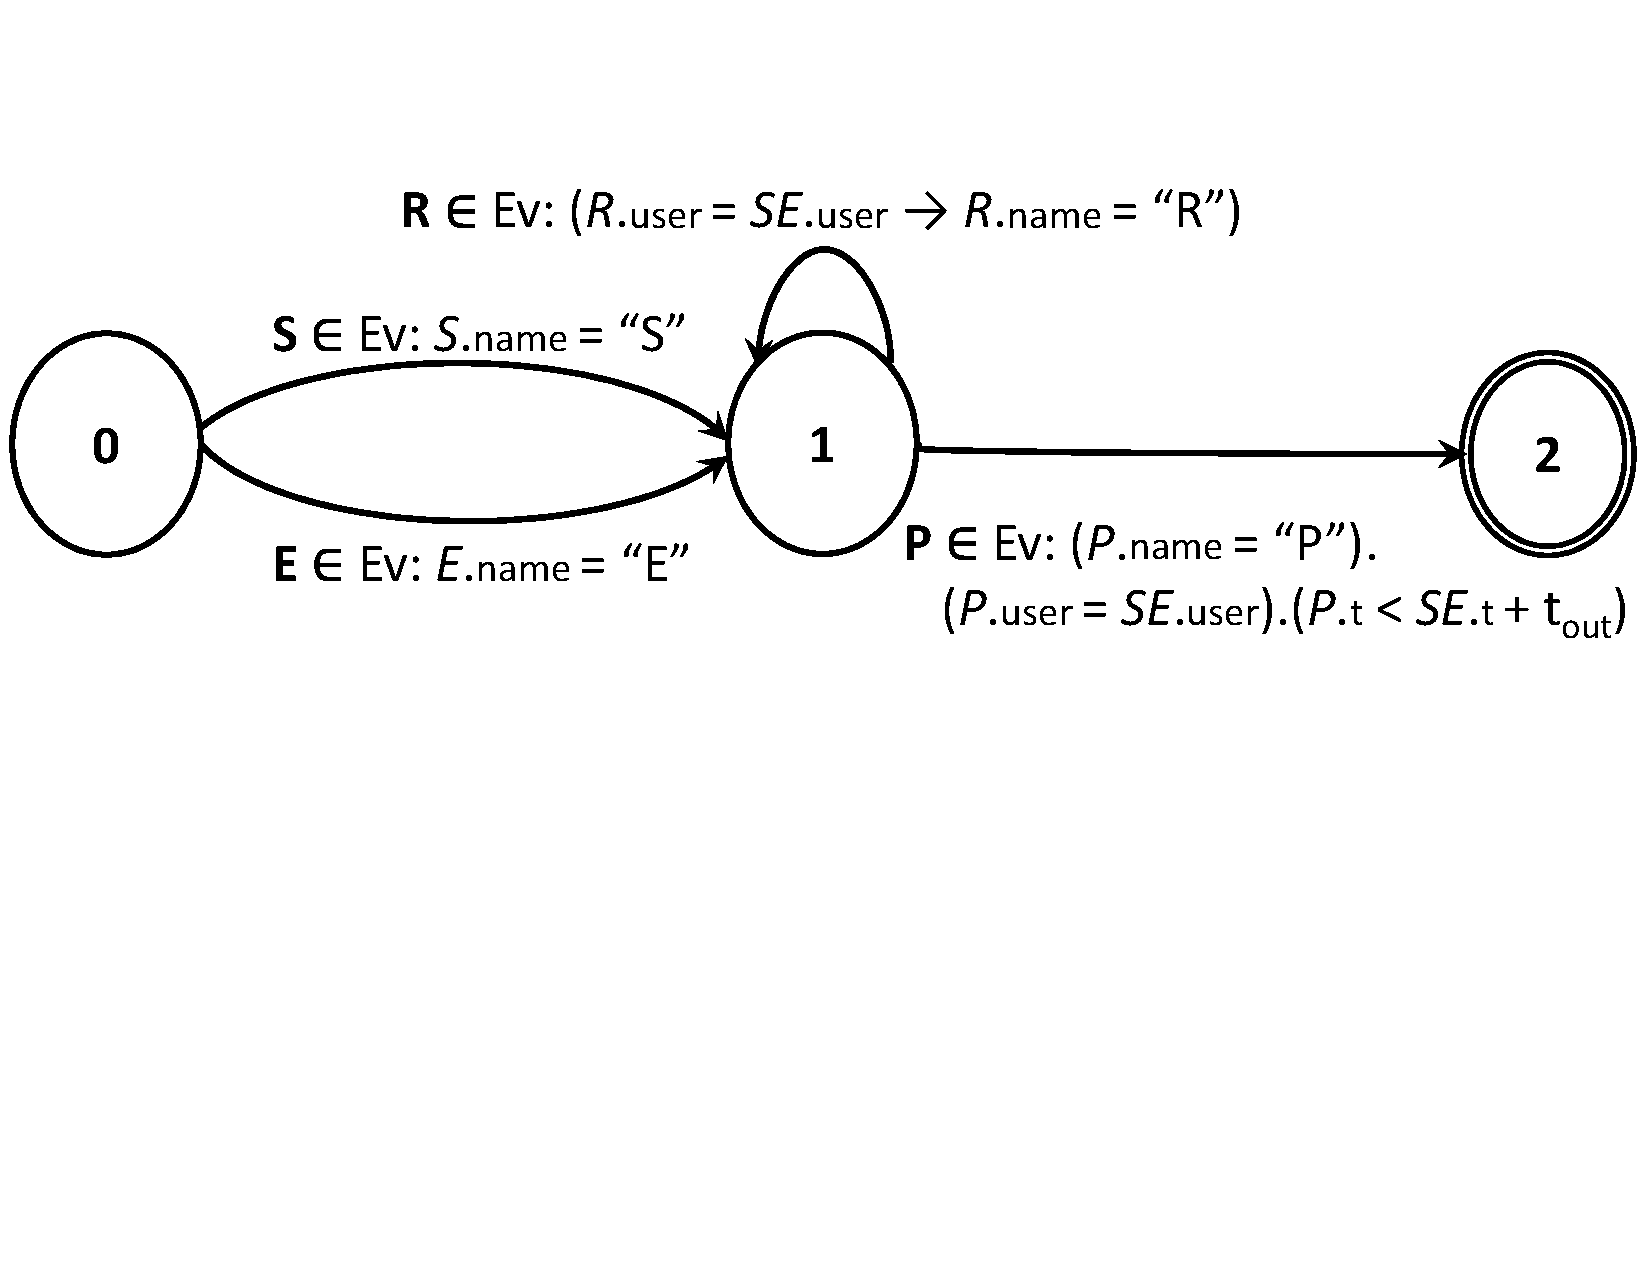
\includegraphics[clip, trim=0cm 10cm 0cm 3cm,width=\columnwidth]
	{graphs/example_sm3.pdf}
	\caption{Automata for the (S|E)R*P pattern.}
	\label{fig:serp_pattern}
\end{figure}


We formally define a finite automaton as $\cA = (S, T, s_{start}, C),$ 
where $S$ is the set of states, $T$ is the set of transitions, $s_{start}$ is 
the initial state and $C$ is the set of completion (accepting) states.
Each transition is defined in terms of the tuple $(X, p_X, src, dst)$ where $X$ 
is the variable binding the event currently considered by that transition, 
$p_X$ is the guard (a propositional formula) 
deciding whether the transition can be triggered or not, and $src$ and $dst$ 
are the transition's source and destination states.  
The atomic formulas of the guard are either {\em selection} predicates, which 
only reference the variable associated with the current transition,
or {\em join} predicates, which may also reference the variables of preceding 
transitions.
In particular, the guards of start transitions can only use selection 
predicates.  


The translation to relational expressions are not limited to 
acyclic automata, but also to automata with cycles of fixed length, 
i.e.\ each iteration of the cycle has the same number of transitions.
This class of automata is of particular importance as it covers the 
vast majority of patterns found in benchmarks and in industrial workloads.  




{\bf Notation.}
We usually denote states by indices $i, j, k$, and we abuse notation to refer 
to transitions using the variable name they introduce (eg. $X, Y, Z$).
In addition we refer to states and transitions also as nodes and edges, 
respectively, in the corresponding graph of an automaton.

To streamline the presentation we begin by considering automata with only
cycles of length 1 and we distinguish between cycle transitions and
non-cycle transitions.


The translation process produces one relational query $Q_i$ per state $i$, and 
the final relational expression of the automata is obtained by unioning all the 
queries generated for the automata's accepting nodes.
Evaluating query $Q_i$ over a set of events computes partial matches, i.e.\ 
sequences of events, corresponding to all the possible paths between the 
starting node and node $i$.
Therefore, if $i$ is the starting node then its query returns an empty sequence 
while if $i$ is an accepting node then it returns complete matches found in the 
input stream of events.
Moreover, the partial (complete) matches computed by $Q_i$ do not include the 
events matched against cycle transitions therefore have a bounded length. 

The schema of the queries we generate consist of a sequence of event variables, 
one for each non-cycle transition that may occur along its associated set of 
paths. 
If a transition is triggered within a partial match, then its corresponding 
variable is initialized by the event that triggered it, otherwise that variable 
is assigned null.
For our example, the schema of query $Q_2$ consists of $S$, $E$ and $P$, and 
for each of its output tuples either $S$ or $E$ is set to null.


State queries $Q_i$ are defined as the union of transition queries $Q_X$ over 
all the incoming non-cycle transitions into state $i$, where each transition 
query $Q_X$ computes partial matches corresponding to the paths ending with 
transition $X$.
In turn, the $Q_X$ query corresponding to a non-starting, non-cycle transition 
is defined as the join between node query $Q_k$, where $k$ is the source of the 
transition, and the input relation of events, where each event considered is 
bound by variable $X$.
The condition enforced by $Q_X$ consists of the guard $p_X$ along with the 
constraint that the timestamp of $X$ succeeds the last event in the partial 
match produced by $Q_k$.
Additionally, a nested query ensures that no other events 
exist between the last event matched by $Q_k$ and the event bound by $X$, 
except for events matching cycle transitions starting and ending in $k$.
By contrast, for starting transitions we only need to apply the transition's 
guard $p_X$ over the input relation.

The translation process iterates in topological order over the nodes of the DAG
obtained by ignoring the cycle transitions of the automaton.
At each node $i$, it first generates the queries for all its incoming
non-cycle transitions $Q_X$ and then $Q_i$ is defined as their union. 
The schema of $Q_i$ is established as the union of the schemas of the incoming 
transitions $Q_X$.

Applying the procedure outlined above to our example produces the following 
queries:
\begin{align*}
%Q_0 =& \{\tuple{}\}
%\quad
Q_S\!=& \{ S \mid S \in \Ev : p_S \}
\;\;
Q_E\!= \{ E \mid E \in \Ev : p_E \}
\;\;
Q_1\!= Q_S \cup Q_E
\\
Q_P\!=& \{ \tuple{SE,P} \mid SE \in Q_1, P \in \Ev:
p_P\ .\ (\facc{SE}{t} < \facc{P}{t}) . 
\\
& 
\qqquad\quad
\{ R \mid R \in \Ev : \facc{R}{t} \in (\facc{SE}{t}, \facc{P}{t})\ .\ 
						! p_R \} = \emptyset
 \}
\\
Q_2\!=& Q_P
\end{align*}

{\bf Translating multi-transition cycles} of fixed length 
($\geq 1$) to relational queries
requires that we first normalize them such that each cycle
has a single starting node and a single ending node, and that the two coincide.
A starting node for a cycle is defined as the destination of one of its 
incoming edges, while an ending node is the source of one of its outgoing edges.
Cycles of fixed length cannot have transversal edges (paths), 
i.e.\ edges (paths) that connect non-adjacent nodes in the cycle, as this would 
violate the restriction that each of the cycle's iterations has the same length.


Given an automaton with a cycle that has multiple starting and ending nodes 
we first duplicate the cycle for each additional starting node. 
Then, for the resulting cycles we duplicate the path between their starting 
node and their last ending node (i.e.\ the furthest from the starting node).  
Finally, we change the source of each outgoing edge to the corresponding 
node in the newly created path, resulting in a cycle whose incoming and 
outgoing edges have the same node as destination and source, respectively.
By applying this procedure to every cycle with multiple starting and ending 
nodes we obtain a normalized automaton.  
While the resulting automaton may have multiple cycles starting 
and ending with the same node, all of those must also have the same length.


The only part of the translation process that changes when generalizing from 
automata with single edge cycles to normalized automata is the specification of 
non-cycle transition queries $Q_X$, and in particular, the specification of its 
nested query should the source state $k$ of $X$ be the starting/ending point of 
a cycle.
We recall that in the case of cycles with a single transition $Y$ the nested 
query enforces that all events occurring in the interval between the last event 
in the partial match computed by $Q_k$ and the timestamp of event variable $X$ 
satisfy guard $p_Y$. 
By contrast, in the case of multi-transition fixed length cycles, for each 
event in the same interval we establish its position (based on  the count of 
events with smaller timestamps) and we ask that it satisfies the guard of the 
transition corresponding to that position in the cycle modulo the length of the 
cycle.
If multiple cycles initiate and conclude at the same node, we alternatively 
have to enforce that all events in an iteration satisfy the corresponding 
transition guards of a particular cycle.


\subsection{Precise filter generation}
\label{sec:prec_filter_generation}



After translating patterns into relational queries a host of relational 
optimizations become applicable, from column pruning and partial aggregation to
the selection of specific join algorithms.
In the following we detail our proposal for speeding up pattern matching in a 
distributed environment based on its representation in the relational world as 
a series of unions and joins.
The first step in this process is to derive a {\em precise} filter which 
retains from the input relation only those events guaranteed to appear in a 
successful match.
While it is understood that constructing and applying such filters may prove 
too expensive to evaluate directly, we discuss them nonetheless as they are 
essential in guiding the design of the {\em abstract} filter, its time and 
space efficient variant. 



% Even though this representation may prove too expensive to evaluate directly, 
% we use it as a stepping stone for building filters designed to discard from 
% the input (almost) all the events that do not participate in a complete match 
% and thus vastly reduce the number of events ultimately processed by the 
% pattern matching engine.
 
% discuss difference between fields referenced by selection predicates and 
% fields referenced by join predicates, and how the symbolic filters are 
% concerned with the latter.






The precise filter of an automaton $\cA$ consists of multiple components, one 
for each of its transitions, and an input event is rejected if it does not 
satisfy any of these components. 
In current work we derive precise filters only for non-cycle transitions and 
single-edge cycles, since the filters for transitions in multi-edge cycles 
are impractical to build/apply and abstract over, as they require the position 
of the considered event within a particular time interval.
 

The precise filter $\precs{X}$ corresponding to a non-cycle transition $X$ of 
automaton $\cA$ is extensionally defined in terms of the events 
from the input that bind the event variable $X$ in the output of its 
semantically equivalent relational query $Q_{\cA}$. 
Therefore $\precs{X}$ can be obtained from the definition of $Q_{\cA}$ by 
projecting away (i.e.\ existentially quantifying) all the other event variables 
in its output besides $X$. 
In our running example the precise filter derived for transition $P$ is:
\begin{align*}
&\precs{P}(P) \equiv \exists SE \in Q_1:
p_P\ .\ (\facc{SE}{t} < \facc{P}{t})\ . 
\\ 
&\qqquad\quad
\{ R \mid R \in \Ev : \facc{R}{t} \in (\facc{SE}{t}, \facc{P}{t})\ .\ 
! p_R \} = \emptyset
\end{align*}

The precise filter $\precs{Y}$ of a cycle transition $Y$, with node $k$ as 
source 
and destination, selects from the input those events that occur within interval 
$(t_Z, t_W)$, where $t_Z, t_W$, are the timestamps of a pair of event variables 
$Z, W$, from the output of $Q_{\cA}$ such that $Z, W$ are associated to 
non-cycle transitions entering and respectively exiting $k$.
$\precs{Y}$ does not need to enforce the guard $p_Y$ as it is 
guaranteed
that all events between $t_Z$ and $t_W$ satisfy $p_Y$ based on the
nested query generated as part of the definition of $Q_W$ (and which was found 
to hold during the evaluation of $Q_{\cA}$).
For the cycle transition $R$ in our example we generate the following filter:
\begin{align*}
\precs{R}(R) \equiv \exists \tuple{SE,P} \in Q_{\cA}: 
 \facc{R}{t} \in (\facc{SE}{t}, \facc{P}{t})
\end{align*}
   



\begin{comment} 
The two kinds of transitions (cycle vs non-cycle) generate distinctly different 
kinds of symbolic filters. 
While both make use of the relational query $Q_{\cA}$ generated for the 
automaton, only the filter for cycle transitions makes direct use of its results
while the other simply uses $Q_{\cA}$'s expression as a starting point for its 
definition.
This distinction plays an important role in how we go about building these 
filters in a distributed environment.
\end{comment}


We take a bottom-up approach to building the filters as it allows us 
to outline an evaluation strategy that operates over sets and which uses set 
operations like union, intersection, set membership or emptiness testing. 
Adopting such a set-centric evaluation strategy is advantageous in a 
distributed environment due to the embarrassingly parallel nature of many set 
operators, but more importantly it gives us a powerful knob in terms of the set 
representations that we use, making it possible to trade off precision in favor 
of performance. 
This strategy is what ultimately guides the design of {\em abstract} 
filters (discussed in sections~\ref{sec:data_abstraction} 
and~\ref{sec:pred_abstraction}), which make our solution practical.
   

As a first step we build a {\em symbolic set} $\syms{X}$ for every transition 
variable $X$ of an automaton $\cA$, 
which collects the values of $X$'s fields joined throughout all the transition 
guards of $\cA$, as $X$ is bound to the input events that satisfy $p_X$'s
selection predicates.
We then re-write the precise filters by replacing each event variable and 
selection predicate associated to a transition with its corresponding symbolic 
set.
Finally, the join predicates get re-written in terms of slicing, intersection 
and emptiness testing over these sets.

The process is showcased in section~\ref{sec:mot_example} where we derive 
symbolic sets $\syms{S}, \syms{R}$ and $\syms{P}$, which we then use in the 
definition of precise filters $\precs{S}, \precs{R}$ and $\precs{P}$ along with 
slicing operators that express the join predicates of the pattern.
We omit the minute technical details of turning transition guards into 
expressions over symbolic sets as they are not particularly challenging.
It involves turning the guards into disjunctive normal form, and replacing in 
each conjunct the transition variables and their selection predicates with the 
corresponding symbolic set, and finally using slicing to encode their join 
predicates.    

\subsection{Data abstraction}
\label{sec:data_abstraction}


Building the precise filters as described in the previous section is not a 
feasible option, as it would require at least just as much work as computing 
the final result (for eg., for $\precs{R}$).
Nonetheless, the precise filters provide a template for designing 
appropriate set abstractions that support the set operations required for 
constructing and querying them in a time and space efficient manner. 
Our approach is to use set abstractions that sacrifice precision, while 
remaining conservative, as we should never eliminate events that would 
otherwise have contributed to a successful match.
We call the resulting structures {\em abstract} filters as they are the outcome 
of employing several abstractions during the process outlined for deriving the 
precise filters.  


First, sets we abstract over contain tuples as 
opposed to single values, where each tuple field holds the values relevant to a 
particular join predicate. 
Similarly, the abstractions we chose need to be multidimensional in the sense 
that they must allow the testing of the domain of values corresponding to a 
specific join predicate, independent of the others.  
Second, we note that besides supporting set intersection and set union, the 
choice for a particular set abstraction is deeply influenced by the particular 
kind of predicates said abstractions needs to support.
For example, in the case of equality joins an appropriate data abstraction 
would be to use Bloom filters as they provide a low cost solution for testing 
whether o value belongs to a set, with the guarantee of no false negatives.
For enforcing inequality joins on the other hand, an interval map, i.e.\ a 
bit vector where each bit stands for a particular interval in the domain,
provides a similarly low cost abstraction.  

Finally, depending on whether the symbolic sets are tested for non-emptiness or 
emptiness, their abstraction has to provide either an over- or an 
under-approximation of the original contents.
For instance, when abstracting over the precise filter $\precs{S}$ from the 
example in section~\ref{sec:mot_example}, we have to use over-approximating set 
abstractions for $\syms{S}$, while the opposite is true for $\syms{\oR}$.
While this is of no concern for set abstractions, like interval maps, which 
support both, it does pose a challenge to abstractions based on hashing, like 
Bloom filters, which can only provide over-approximations.


One way to address the issue raised by hash-based data abstraction wrt.\ sets 
that require under-approximation is to replace them with the coarsest 
under-approximation possible, i.e. the empty set $\emptyset$ (as showcased in 
section~\ref{sec:mot_example}).
Alternatively, one can re-write the precise filter using min aggregates:
\begin{align*}
&
\PrecedesPP(\symv{s}) \equiv 
\min \{ 
\facc{\symv{p}}{t} \mid 
\symv{p} \in 
\slice{\syms{P}}
{(\facc{\symv{s}}{t}\,:\,\facc{\symv{s}}{t} + t_{out}),\; 
	\facc{\symv{s}}{user}}
\}
\\
&\qquad\;\;\,
< \min \{ 
\facc{\symv{r}}{t} \mid 
\symv{r} \in 
\slice{\syms{\oR}}
{(\facc{\symv{s}}{t}\,:\,\facc{\symv{s}}{t} + t_{out}),\; 
	\facc{\symv{s}}{user}} 
\},
\end{align*}
which captures the fact that a Search event is part of a complete match if the 
next Purchase event precedes the next event different from Read-review.
Now, we can safely use hashing to abstract over user ids as follows:
\begin{align*}
&
\PrecedesPP^{\hashid{user}}(\symv{s}) \equiv 
\\
&\qquad\;\;\;\,
\min_{u \in \hashid{\facc{s}{user}}}
\min \{ 
\facc{\symv{p}}{t} \mid 
\symv{p} \in 
\slice{\syms{P}}
{(\facc{\symv{s}}{t}\,:\,\facc{\symv{s}}{t} + t_{out}),\; 
	u}
\}
\\
&\qquad
< 
\max_{u \in \hashid{\facc{s}{user}}}
\min \{ 
\facc{\symv{r}}{t} \mid 
\symv{r} \in 
\slice{\syms{\oR}}
{(\facc{\symv{s}}{t}\,:\,\facc{\symv{s}}{t} + t_{out}),\; 
	u} 
\}.
\end{align*}

While for this example it was possible to come up with an alternative 
formulation of the precise filter, this may not always be the case. 
And even if it is possible, the alternatives may be too expensive to
materialize and query (for eg.\ evaluating $\PrecedesPP^{\hashid{user}}$ can 
easily be more costly than $\PrecedesP^{\interval{t}}$).
Therefore, in the next section we discuss how {\em predicate abstraction} can 
mitigate these kinds of issues.

\subsection{Predicate abstraction}
\label{sec:pred_abstraction}


We propose {\em predicate abstraction}, ie.\ the technique of weakening
 the
precise filters by discarding some of their predicates, as a way of
 overcoming
the challenges that can arise when turning them into abstract 
filters.
For example, it may happen that for some predicate types
(for eg.\ $x.Contains(y)$, where $x$, $y$ are strings) we simply cannot
 provide
any data abstraction, and even for those that we can, materializing and
 querying
those data abstractions might prove too expensive.




Predicate abstraction is an essential component of our approach
allowing us to strike the right balance between the data reduction that the
abstract filters provide on one hand, and the overheads introduced by their
data abstractions on the other.
For instance, we may choose to discard
predicates that have very low selectivity, i.e.\ the reduction in input 
data
that they provide does not justify the cost of enforcing them.
Similarly, one may turn to predicate abstraction when dealing with patterns
 with
a large number of join predicates or transitions, in order to mitigate the
increased overheads incurred by their data abstractions.


Given a join predicate $\theta(X.f, Y.f)$, the definition of precise filter 
$\precs{X}(\symv{x})$ is bound to contain a corresponding slicing of $Y$'s 
symbolic set as $\slice{\syms{Y}}{...,f}$. 
Just like in the case of data abstraction, depending on whether predicate 
$\theta$ appears in a negated sub-clause or not, its abstraction needs to be 
under or over approximating, in order to preserve conservativeness.
More precisely, we enforce the over-approximation of $\theta$ by assuming that 
the $f$ dimension of $\syms{Y}$ is invariably the entire domain of $f$.
Analogously, the under-approximation of $\theta$ leads to the assumption that 
the $f$ dimension of $\syms{Y}$ is invariably void, which by consequence 
reduces the entire $\syms{Y}$ to the empty set.
In section~\ref{sec:mot_example}, it was the under-approximating abstraction of 
predicate $\facc{S}{user} = \facc{R}{user}$ that produced the relaxed filter
$\PrecedesPPP$, by turning $\syms{\oR}$ in $\PrecedesP$ to the empty set.  
 
Finally, we remark that predicate abstraction need not be applied symmetrically,
i.e.\ given join predicate $\theta(X.f, Y.f)$ one could choose to abstract over 
$\syms{X}$'s $f$ dimension but not over the $f$ dimension of $\syms{Y}$, or 
vice-versa.  
This can prove useful if one of the symbolic sets is known to be a subset of 
the other, thus one would need to build an abstract filter only for the smaller 
one. 
Moreover, considering that initial or final transitions typically have the 
fewest number of matching events, one might choose to only collect and abstract 
over the symbolic sets of those transitions.
Due to their low cardinality these sets are likely to have very high 
filtering power and the data abstractions used to enforce them can achieve 
higher precision for the same operating costs (considering the small number of 
values to store and query).
Applying this heuristic to our example from section~\ref{sec:mot_example} wrt.\ 
to the final transition P (as we expect to have relatively few purchasing 
events) produces the following relaxed filters:
\begin{align*}
\heurs{S}(\symv{s}) 
&\equiv  
\slice{\syms{P}}
{(\facc{\symv{s}}{t}\,:\,\facc{\symv{s}}{t} + t_{out}),
	\facc{\symv{s}}{user}} 
\neq \emptyset
\\
\heurs{\oR}(\symv{r}) 
&\equiv
\slice{\syms{P}}{(\facc{\symv{r}}{t}\,:\,\infty), \facc{\symv{r}}{user}}
\neq \emptyset
\\
\heurs{P}(\symv{p}) 
&\equiv \texttt{true},
\end{align*}
as obtained 
from the definitions of $\precs{S}, \precs{\oR}$ and $\precs{P}$
by replacing $\syms{S}$ with the full domain of time/user ids and  
$\syms{\oR}$ with the empty set. 
By further applying data abstraction to these filters, we end up with a 
relatively cheap way to dispose of a large number of the input events, 
irrelevant to our pattern.  

\subsection{Building filters through fixpoint}


We remark that the abstract filters are not strictly tied to the  
expressibility of automata as relational queries, but that they can also be 
computed for an arbitrary automaton by using a fixpoint operator that keeps 
track of provenance information.
The fixpoint operator we consider assigns to the starting node the empty 
sequence and then iteratively builds for every node of the automaton its 
corresponding set of (partial) matches, until no more new matches are found. 
In every iteration, for each node $i$ and each of its outgoing transitions $X$, 
the partial matches added by the previous round to $i$ get extended if matching 
events are found within the symbolic set of $X$. 
The newly found matches then get added to the collection of matches 
corresponding to $X$'s destination, and the process starts over.  
Since we never remove partial matches we are guaranteed to reach a fixpoint.
Based on the complete matches collected by the accepting nodes, we also update 
the abstract filter's components corresponding to the transitions along their 
path.

In designing the fixpoint operator we similarly make extensive use of sets and 
set operators.
In particular, the (partial) matches we compute for each node $i$ of the 
automaton are represented as a sequence of sets, one for each transition that 
may occur on a path from the start node to $i$.
Then the abstract filter for a specific transition can be obtained by unioning 
its corresponding set across all the accepting nodes.
When deciding whether a partial match can be extended by triggering transition 
$X$, we simply intersect the symbolic set $\syms{X}$ with the projection from 
the partial match of the corresponding join fields, i.e.\ those fields of 
previously occurring transitions that are joined against $X$.
If the result is empty then the extension is not possible, otherwise a new 
partial match gets created whose corresponding set for transition $X$ is the 
result of the intersection.   





 
